\documentclass[journal]{IEEEtran}

\usepackage{cite}
\usepackage[pdftex]{graphicx}
\usepackage{float}



\begin{document}


\title{Optimization}

\author{Rodrigo Caye Daudt}

% The paper headers
\markboth{Optimization}%
{Rodrigo Caye Daudt}


% make the title area
\maketitle


\begin{abstract}
%\boldmath
This describes the implementation and results of several minimization/optimization methods. The methods are divided in three groups: 1D, 2D, and ND inputs.
\end{abstract}




\IEEEpeerreviewmaketitle


%%%%%%%%%%%%%%%%%%%%%%%%%%%%%%%%%%%%%%%%%%%%%%%%%%%%%%%%%%%%%%%%%%%%%%%%%%%%%%%%
%%%%%%%%%%%%%%%%%%%%%%%%%%%%%%%%%%%%%%%%%%%%%%%%%%%%%%%%%%%%%%%%%%%%%%%%%%%%%%%%
\section{Introduction}

\IEEEPARstart{F}{unction} optimization is a field of mathematics that deals with the search of the input element of a function that yields the output that best conforms with some predefined criteria. This seach has many applications throughout different scientific fields, from economics to control engineering. Some applications of function minimization are the training of neural networks, simultaneos localization and mapping (SLAM), and real time optimization (RTO) control.

Several different methods of function optimization are presented in the following sections. These methods are described and compared, focusing on pratical aspects such as complexity, convergence issues and issues with logal minima.




%%%%%%%%%%%%%%%%%%%%%%%%%%%%%%%%%%%%%%%%%%%%%%%%%%%%%%%%%%%%%%%%%%%%%%%%%%%%%%%%
%%%%%%%%%%%%%%%%%%%%%%%%%%%%%%%%%%%%%%%%%%%%%%%%%%%%%%%%%%%%%%%%%%%%%%%%%%%%%%%%
\section{Code Glossary}

The code that was used to exemplify and evaluate the optimization methods presented later in this paper were programmed using MATLAB. The files can be divided in two groups, functions and scripts. Next is a glossary of the files contained in this work



%%%%%%%%%%%%%%%%%%%%%%%%%%%%%%%%%%%%%%%%%%%%%%%%%%%%%%%%%%%%%%%%%%%%%%%%%%%%%%%%
%%%%%%%%%%%%%%%%%%%%%%%%%%%%%%%%%%%%%%%%%%%%%%%%%%%%%%%%%%%%%%%%%%%%%%%%%%%%%%%%
\section{Minimization In 1D}

Text text


\begin{figure}
\centering
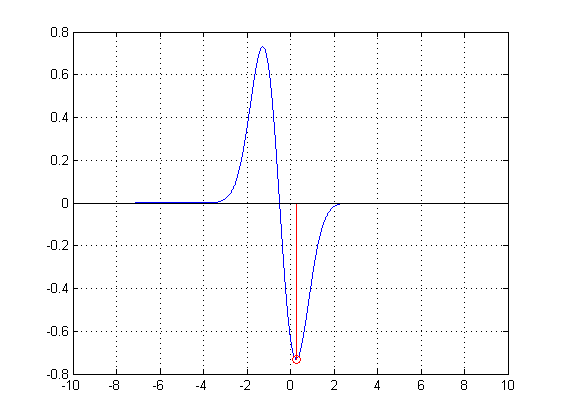
\includegraphics[width=3.4in]{figures/1d-bruteForce.png}
\caption{}
\label{figBF}
\end{figure}

\begin{figure}
\centering
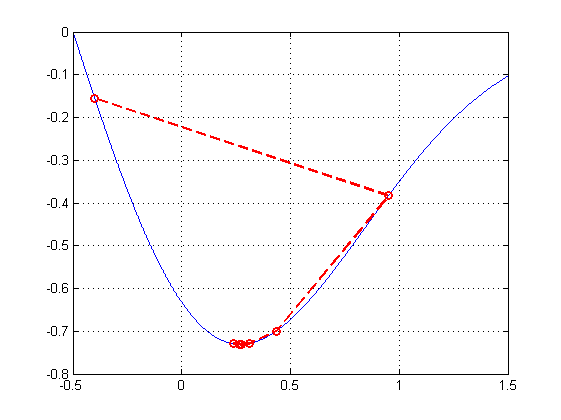
\includegraphics[width=3.4in]{figures/1d-goldenSearch.png}
\caption{}
\label{figGS}
\end{figure}

\begin{figure}
\centering
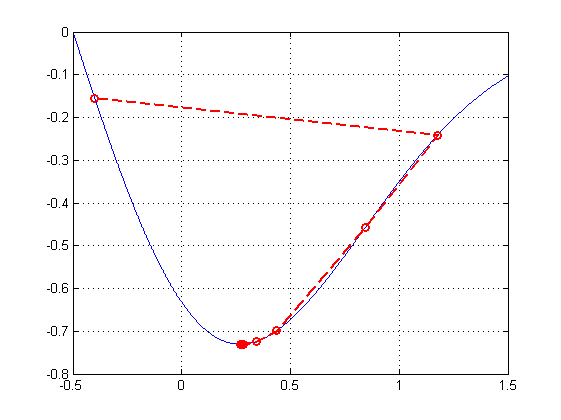
\includegraphics[width=3.4in]{figures/1d-brentsMethod.png}
\caption{}
\label{figBM}
\end{figure}

\begin{figure}
\centering
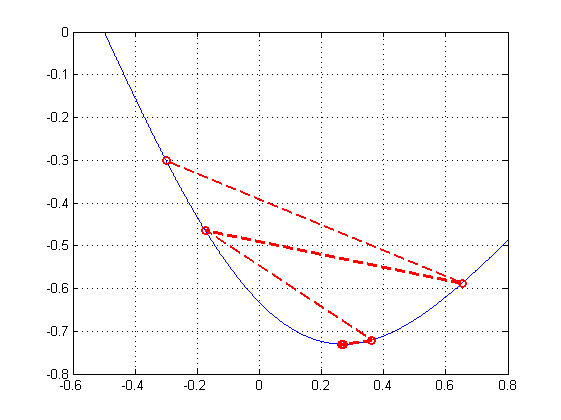
\includegraphics[width=3.4in]{figures/1d-newtonsMethod.png}
\caption{}
\label{figNM}
\end{figure}


%%%%%%%%%%%%%%%%%%%%%%%%%%%%%%%%%%%%%%%%%%%%%%%%%%%%%%%%%%%%%%%%%%%%%%%%%%%%%%%%
%%%%%%%%%%%%%%%%%%%%%%%%%%%%%%%%%%%%%%%%%%%%%%%%%%%%%%%%%%%%%%%%%%%%%%%%%%%%%%%%
\section{Minimization In 2D}

\subsection{1}

Aaa

\begin{figure}
\centering
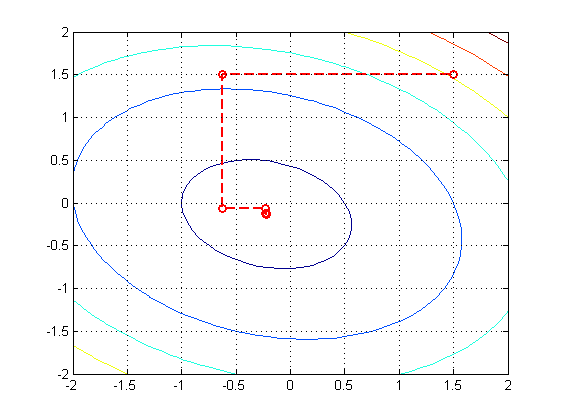
\includegraphics[width=3.4in]{figures/2d-arbitraryLineSearch.png}
\caption{}
\label{figALS}
\end{figure}

\begin{figure}
\centering
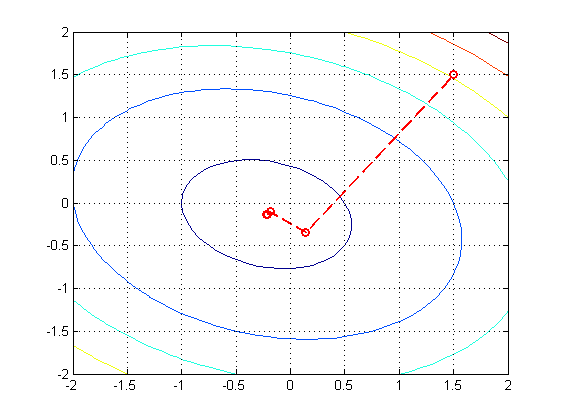
\includegraphics[width=3.4in]{figures/2d-steepestDescent.png}
\caption{}
\label{figSD}
\end{figure}

\begin{figure}
\centering
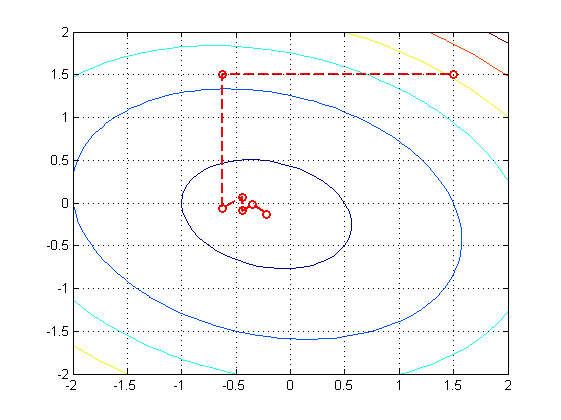
\includegraphics[width=3.4in]{figures/2d-powellsMethod.png}
\caption{}
\label{figPM}
\end{figure}

\begin{figure}
\centering
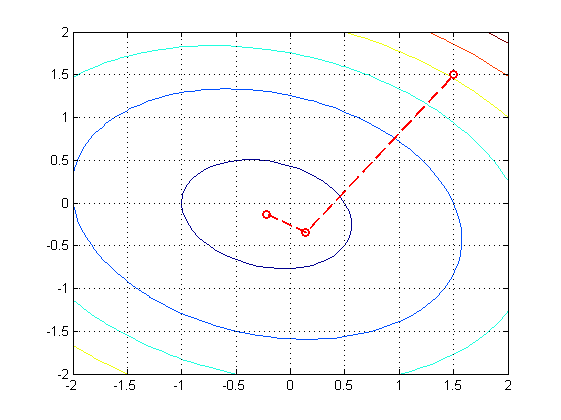
\includegraphics[width=3.4in]{figures/2d-conjugateGradient.png}
\caption{}
\label{figCG}
\end{figure}

\subsection{2}

Aaa

\begin{figure}
\centering
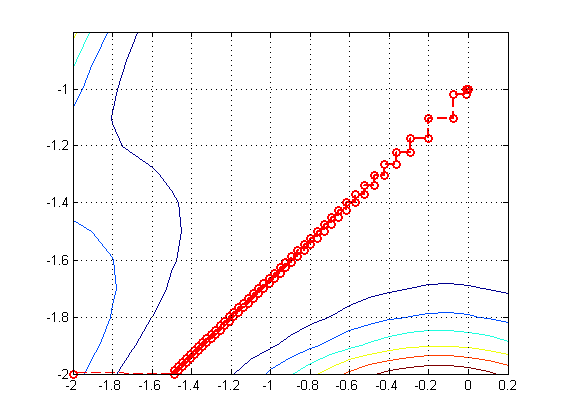
\includegraphics[width=3.4in]{figures/2d2-arbitraryLineSearch.png}
\caption{}
\label{figALS2}
\end{figure}

\begin{figure}
\centering
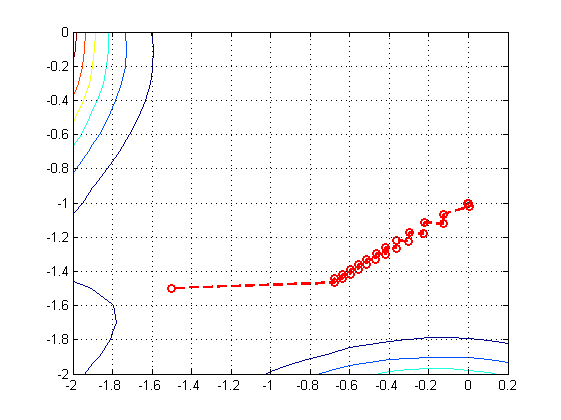
\includegraphics[width=3.4in]{figures/2d2-steepestDescent.png}
\caption{}
\label{figSD2}
\end{figure}

\begin{figure}
\centering
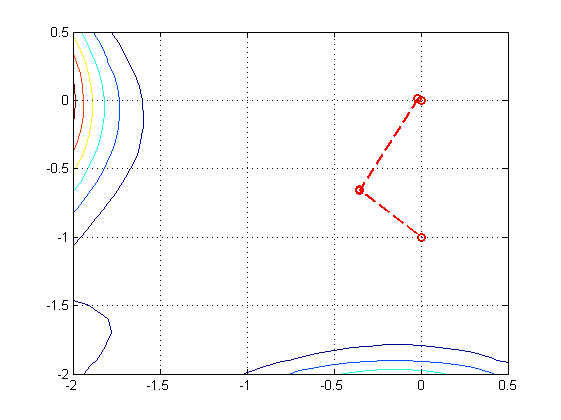
\includegraphics[width=3.4in]{figures/2d2-quasiNewton.png}
\caption{}
\label{figQN}
\end{figure}


%%%%%%%%%%%%%%%%%%%%%%%%%%%%%%%%%%%%%%%%%%%%%%%%%%%%%%%%%%%%%%%%%%%%%%%%%%%%%%%%
%%%%%%%%%%%%%%%%%%%%%%%%%%%%%%%%%%%%%%%%%%%%%%%%%%%%%%%%%%%%%%%%%%%%%%%%%%%%%%%%
\section{Minimization In nD}

Text text

\begin{figure}
\centering
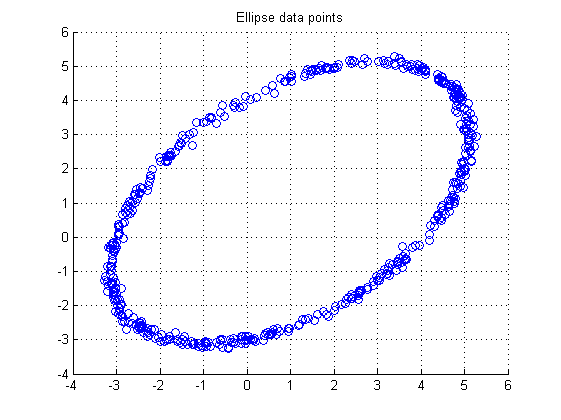
\includegraphics[width=3.4in]{figures/nd-groundTruth.png}
\caption{}
\label{figGT}
\end{figure}

\begin{figure}
\centering
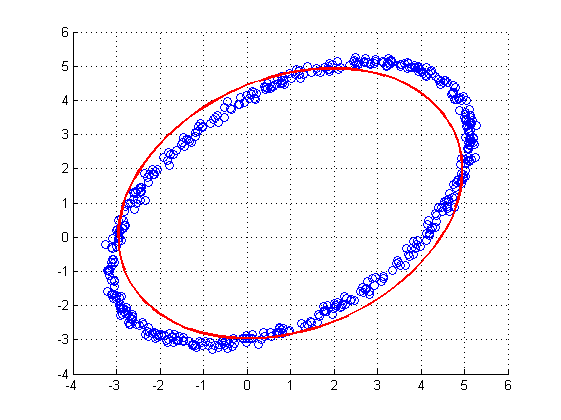
\includegraphics[width=3.4in]{figures/nd-fittedEllipse.png}
\caption{}
\label{figFE}
\end{figure}


%%%%%%%%%%%%%%%%%%%%%%%%%%%%%%%%%%%%%%%%%%%%%%%%%%%%%%%%%%%%%%%%%%%%%%%%%%%%%%%%
%%%%%%%%%%%%%%%%%%%%%%%%%%%%%%%%%%%%%%%%%%%%%%%%%%%%%%%%%%%%%%%%%%%%%%%%%%%%%%%%
\section{Conclusion}
The conclusion goes here.





%%%%%%%%%%%%%%%%%%%%%%%%%%%%%%%%%%%%%%%%%%%%%%%%%%%%%%%%%%%%%%%%%%%%%%%%%%%%%%%%
%%%%%%%%%%%%%%%%%%%%%%%%%%%%%%%%%%%%%%%%%%%%%%%%%%%%%%%%%%%%%%%%%%%%%%%%%%%%%%%%
\bibliographystyle{IEEEtran}
\bibliography{Optimization}

%%%%%%%%%%%%%%%%%%%%%%%%%%%%%%%%%%%%%%%%%%%%%%%%%%%%%%%%%%%%%%%%%%%%%%%%%%%%%%%%
%%%%%%%%%%%%%%%%%%%%%%%%%%%%%%%%%%%%%%%%%%%%%%%%%%%%%%%%%%%%%%%%%%%%%%%%%%%%%%%%
\appendices

\begin{figure*}[p]
\section{Code}
Appendix one text goes here.
\end{figure*}




% that's all folks
\end{document}


